%!TEX root=paper.tex
  
\newpage
\section{Overhead of the \tool}
\label{sec:overhead}

To know the performance overhead of the \tool, we have implemented an automated benchmark system. It is open source and available online and can be tested by the reader. The benchmark does the following steps: 

\begin{itemize}
	\item downloads the latest version of the Zeeguu API and installs it in a Docker container
	\item calls multiple endpoints for 500 times tracking the response times. the endpoints are called in three configurations
	\begin{itemize}
		\item with the dashboard disabled
		\item with the dashboard enabled but with the outlier detection deactivated
		\item with the dashboard enabled and the outlier tracking enabled always
	\end{itemize}
\end{itemize}

\Fref{fig:bench} shows the results of calling every one of the three endpoints for 500 times. 


\begin{figure}[h!]
	\centering
	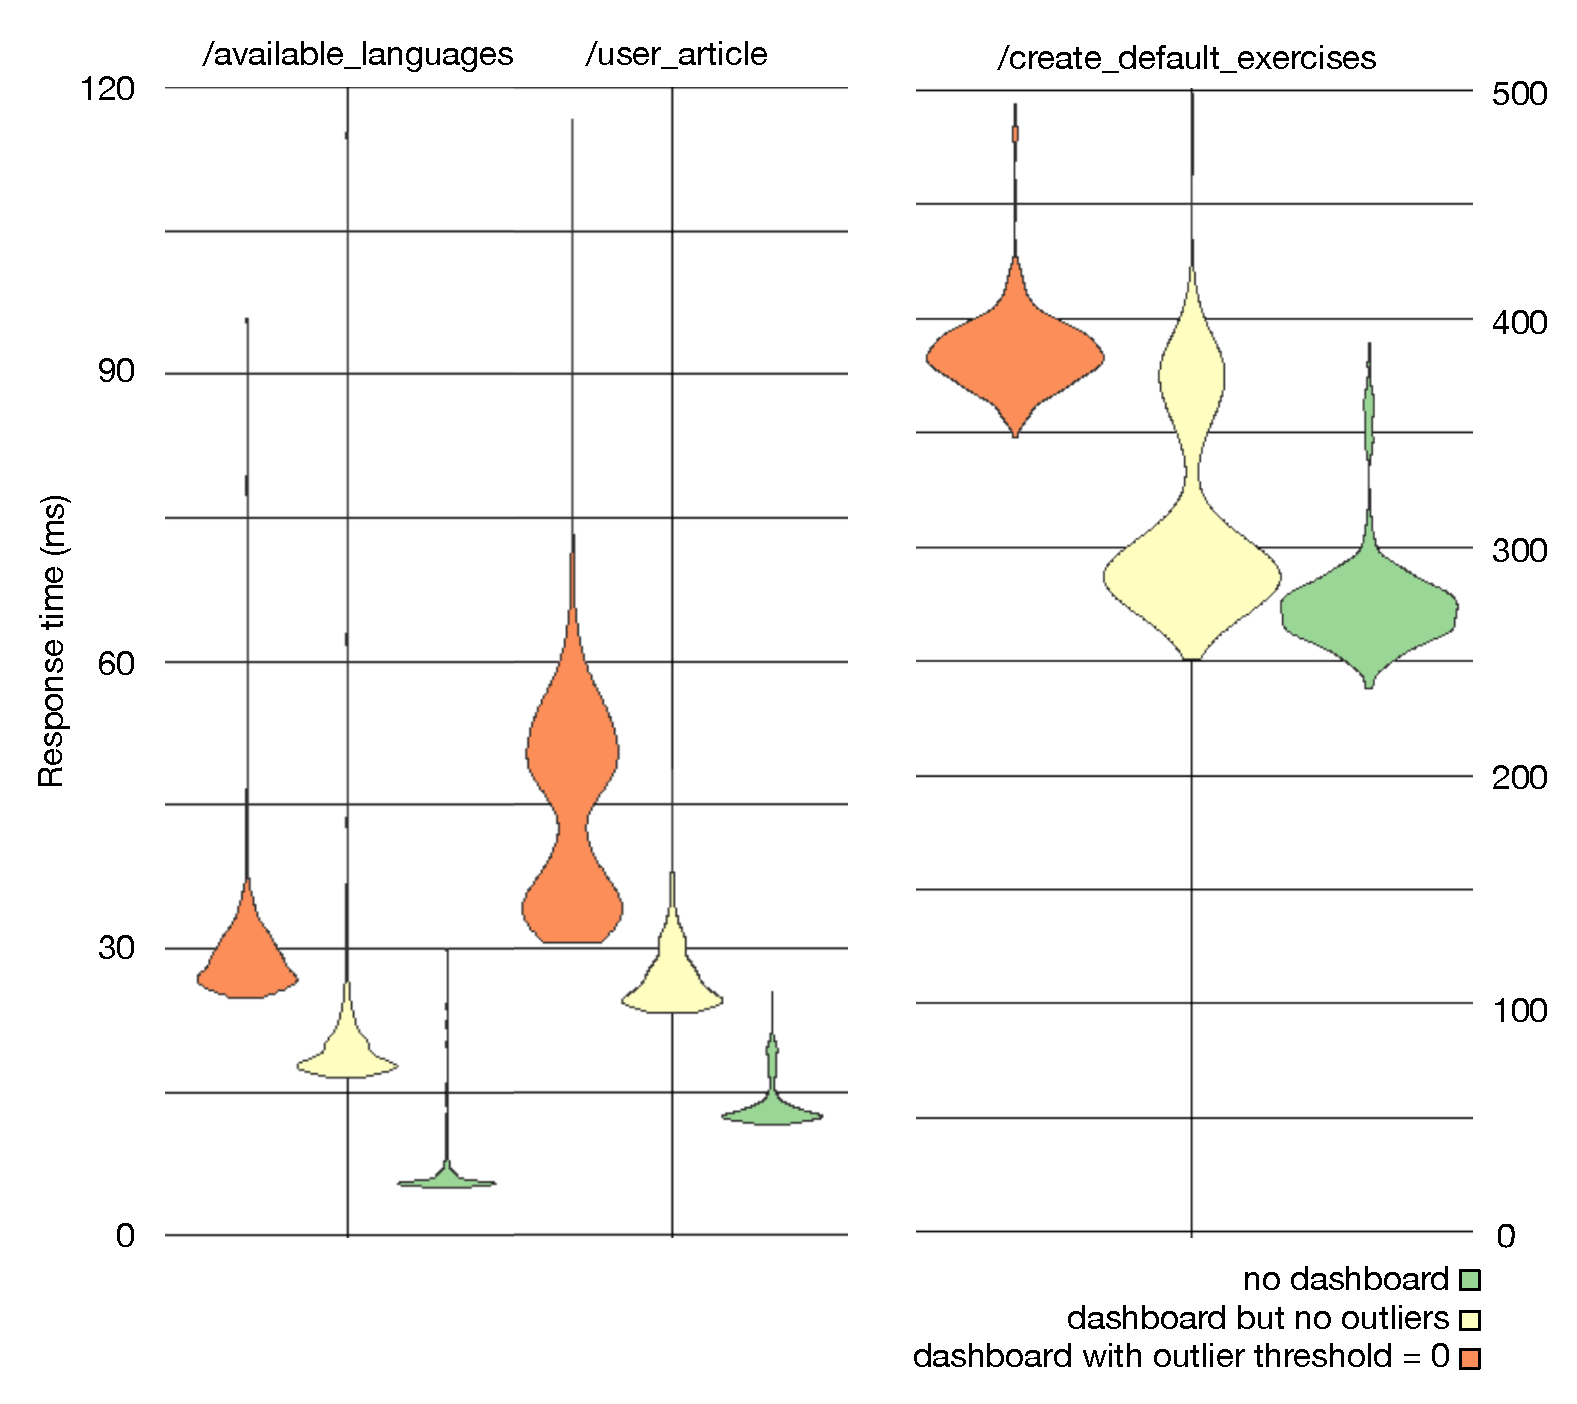
\includegraphics[width=\linewidth]{benchmark2.pdf}
	\caption{The distribution of response times when calling the three endpoints for 500 times in three conditions: no dashboard, dashboard but no outliers, dashboard and always outlier routine}
	\label{fig:bench}
\end{figure}

We run the benchmarking script on a quad-core machine, with Intel Core i5-4590 processor, @ 3.30GHz, 8G of RAM and 240GB SSD disk drive.



Observation -- not easy to benchmark this... it's flask on top of python communicating with 

- this introspection, which looks up endpoints, happens only once at the startup of the service, so it is going to affect the API startup performance, but not the actual endpoint performance. In our case, the overhead here was quite small: TO MEASURE


  